\chapter{Object Tracking} \label{cha:tracking}
This chapter is focused on a few methods that solve the traditional task of object tracking. For each algorithm the potentiality is shown and the advantages, compared to other methods, will be discussed. In addition, an overview of similar problems is given in~\Cref{sec:tracking-conditions}.


\section{Task definition} \label{sec:tracking-definition}
Object tracking is a challenge that, differently from the detection, does not work with images but deal with videos. A video is technically defined as a sequence of images, called \textbf{frames}, combined together at a certain frame rate. Typically this rate is 15, 30 or 60 FPS (Frames Per Second).\\
The interconnection of the frames of videos is used from the object tracker algorithms to create knowledge, based on the previously analysed images, by storing information. An object detector elaborates a picture at a time, each one independently from the other. There is no connection among images of the same database. Instead, a tracker process images one at a time but it uses the knowledge, of the previously analysed frames, to understand the current incoming image.\\
The task baseline is defined as:
\begin{tcolorbox}
	\begin{center}
		\textit{\textbf{The traditional tracking challenge} consists of tracking a single well-defined subject over a short video clip, no matter if it is a person, an animal or an inanimate object. The target of the tracking clearly fully appears into all the frames of the sequence.}
	\end{center}
\end{tcolorbox}


\subsection{Interface}
Structure of the tracking algorithms interface:
\begin{itemize}
	\item One input value is composed of an image, typically the first frame of a video. In our case of real-time elaboration the image corresponds to the actual view of a webcam connected to the device.
	\item The other input corresponds to the bounding box coordinates of the subject that needs to be tracked. The bounding box can be manually generated or can be automatically identified with an object detector.
	\item All future steps get as input a new frame. The task is to understand, in this new image, where is located the subject defined by the initial bounding box.\\
	Then, if all these elaborated images and the generated bounding boxes, are combined together, the result is a video. The initial subject of the video while moving is always centred into a rectangle that follows it across the entire \textbf{FoV (Field of View)} of the camera.
\end{itemize}


\subsection{Scope of the tracking}
It is important to note that the task is called "\textit{Object tracking}" and not "\textit{Person tracking}" this is because there are no limitations to the subject that needs to be tracked, it does not necessarily need to be a human. A better name for the challenge could be "\textit{Area tracking}" because the algorithms should follow the rectangle of coloured pixels that was located in the initial bounding box. No assumption can be done of which type of subject exists inside the bounding box.\\
Generally, these methods work if the initial position is centred around an object that moves consistently in the space and does not change aspect. Some examples that could break these methods are:
\begin{itemize}
	\item The initial bounding box contains two or more objects that move independently from each other. The algorithm will recognise one of the two as the main subject and will track it over the video and lose the other one. \\
	This is a problem if accidentally the bounding box contains something that is "more important" than the "\textit{real subject}". It can also be an advantage that allows to easily discard the background that is an "\textit{object}" itself.\\
	Since two independent objects move differently in the space compared to a single unique object, tracking them can easily create unexpected errors due to inconsistent movements.
	\item The subject changes aspect too rapidly due to different luminosity in the environment, or elaborated video sequences that are not "\textit{natural}". This last possibility often breaks methods designed for real situations, so it is not a problem only in this case. Instead, the change of luminosity often occurs but a solution can be achieved with frame pre-processing, such as the standardization of the luminosity of the image to always process a figure with the same luminosity.
\end{itemize}


\subsection{Deal with special conditions}\label{sec:tracking-conditions}
The tracking task can be seen as a set of problems. This is because there are a lot of conditions that can modify the scenario where the algorithms should work. By modifying the type of difficulties in the videos some methods may fail while others may not.\\
The goal of this thesis is to build a "person tracker", that should work under certain conditions. The problem is that the combination of a lot of requirements makes the problem harder.\\
Despite the time spent for a programmer to ideate, implement and test a solution there is a trade-off to consider. Solving a hard task requires a more computational complex solution compared to solving a similar easier task. This complexity influences the performances of the proposed algorithm. To conclude, it is important to understand which are the requirements of the problem that we are dealing with, in order to choose the algorithm that it is better to use, to solve the task and to perform it fast.\\
\\
Below are listed a set of requirements that make the baseline harder (definition is in~\Cref{sec:tracking-definition}):
\begin{itemize}
	\item \textbf{Changes of 2D shape}: the target due to movements might change its ratio, aspect, and shape. We are interested in what the camera sees of the subject (2D  space) and not the effective actual condition of the subject (3D space).
	\begin{itemize}
		\item \underline{Partial occlusion} (\Cref{fig:challenge_partialOcclusion}): it may happen that during the video, part of the subject is occluded, by an object. If this happens the algorithms must be designed to be robust and to localize the target even with a small section of it.\\
		The bounding box generated may contain only the visible part of the subject but it may also happen that an estimation of the entire subject is done and the bounding box contains both the visible and the estimated missing area of the target.
		\item \underline{Rotations and deformations} (\Cref{fig:challenge_deformation}): the object tracked while moving can rotate and show to the camera a different side, or if it is deformable, change the shape (i.e. a person walking change the shape continuously). This might influence even colours.
	\end{itemize}
	
	\item \textbf{Total occlusion} (\Cref{fig:challenge_totalOcclusion}): the subject completely disappears behind an object or out of the camera field of view.
	\begin{itemize}
		\item \underline{Short-time occlusion}: the subject is hidden for a very small number of frames (i.e. 5 or less). This often happens when the subject or an obstacle is moving and the three elements, subject, object and camera, are aligned. These very short occlusions may be solved using a little memory that stores the subject information for the last few frames (i.e. 10).
		\item \underline{Long-time  occlusion}: the occlusion lasts for a bigger number of frames, even seconds. Often it occurs when the subject exits the field of view of the camera and does not enter it again for a while. It can also happen if the subject is behind a big obstacle such as a vehicle or a wall.\\
		It is harder to solve compared to the previous scenario, because the solution requires a long term memory associated with a recognition procedure to understand when the subject is visible back again.
	\end{itemize}

	\item \textbf{Fast-moving object}: the subject shifts for a big portion of the picture from the old position to the new one in a single frame. Meaning that there was a big 2D movement. This could happen because the subject is effectively moving fast, or because it is close to the camera and even a small movement looks big.
	\begin{itemize}
		\item \underline{Blurred subject} (\Cref{fig:challenge_blurred}): due to its movement the subject is blurred and this heavily changes its aspect. The modified elements are the shape and the colours that are somehow faded. In addition, especially for humans, moving fast can make parts of the body such as arms or legs disappear.
		\item \underline{Proximity assumption} (\Cref{fig:challenge_proximity}): a lot of trackers are based on the assumption that the subject moves around only a little bit. If it moves fast this principle is broken.\\
		After knowing the exact location of the subject on the previous frame starts the estimation on the following one.\\
		At this point there are two things to focus on:
		\begin{itemize}[\ding{228}] %method to insert custom symbol in itemize (\ding(228) = the full >)
			\item If the subject does not move is probable that the prediction will place the target in the exact same position as before. Instead, if it moves the probability that the tracked object will be located close to the previously known position is higher than to be located far away. Specifically, the likelihood can be seen as a \textbf{Multivariate Normal Distribution} centred at the previous position and stretched towards the direction where the subject is moving (\Cref{fig:challenge_multivariate}).
			\item If multiple similar objects exist in the frame and the tracking is following one of them, it is probable to lose it. This happen with a fast movement that generates an unpredictable big shift, and the target moves far away from the previous position while the tracker recognise its subject into a similar object. From now on, the tracking is broken because it follows the wrong physical element.
			\item A big shift can also be wrongly interpreted as a total occlusion.
			\item On the other hand, reducing the tolerance to big movement allows the algorithms to only search locally around the last known position resulting in a big improvement of the overall performance.
		\end{itemize}		
	\end{itemize}

	\item \textbf{Low-resolution images} (\Cref{fig:challenge_lowResolution}): as with many other computer vision challenges the resolution of the input image is fundamental. A low number of pixels per frame results into a bounding box (often a small portion of the entire image) of very low resolution. Because of this, recognising the key elements that identify the subject is hard, but also faster and computationally cheaper.

	\item \textbf{Moving background/camera}: working on a fixed camera allows the use of a set of techniques based on background subtraction. The key idea is to get prior knowledge of the background and understand which objects are there, by removing the known part pixel by pixel. A big change of luminosity can make this harder, but still possible.\\
	A camera that rotates always on the same section can be managed as a fixed camera. This can be done by combining all the images along with the rotation as a unified one, creating a \underline{panorama image}.\\
	Instead, a moving camera implying a moving background makes everything harder:
	\begin{itemize}
		\item No background subtraction can be done.
		\item The subject may change aspect even if it does not move.
		\item The occlusion, both partial and total, can occur more easily.
		\item A zoom or rotation of the camera causes a similar effect such as the "fast-moving object".
		\item To estimate the movement speed and direction of the subject it is necessary to know the movement of the camera because one is relative to the other. However, almost always the displacement of the camera in the space is unknown.
	\end{itemize}

	\item \textbf{Real-time}: designing a method to run in real-time requires to focus on the computational capability and respectively to the processing speed. Real-time might vary from 1 to 60 FPS according to the application. To achieve this speed it is often necessary to choose a faster method instead of an accurate one. This reduces the overall precision of the entire designed algorithm.\\

	\item \textbf{Long-term video sequences}: the input frame sequence is longer than a few seconds, up to minutes. Firstly, a long video might easily contain some of the problems listed above. In addition, trying to locate the same subject over and over again without a reinitialization can fail due to the drift problem.\\
	The \textbf{drift problem} consists of an accumulation of small errors along the tracking period. A tracking algorithm refers to the bounding box generated for the previous frame. The subject that should be located again in the new frame is extracted from that bounding box. If the tracking lasts for a small number of frames, the subject may look similar to the original one. Instead, during a long processing the bounding box starts to derive from the original subject. Due to partial occlusion, the box might be reduced. Due to a strong change of luminosity, the bounding box might be misaligned. Due to a fast movement, the box can be linked to the background. By continuing summing up all these little problems the main subject will be recognised as a superfluous element. Therefore the tracker stops to consider it useful and the track fails.\\
	To solve this problem the solution is to re-initialize the tracker often before reaching the limit of the drift. This can be done with different methods such as a \textbf{Kalman filter} or by recognising the main subject with a detection, that is the method presented in this thesis.
	
	\item \textbf{Multiple subjects} (\Cref{fig:challenge_multiple}): if there is more than a subject to follow the naive solution is to apply an object tracker to each of them. Each tracker works independently from the others therefore given $X$ subjects the performances $f$ measured in FPS are reduced to $f/X$.\\
	An efficient solution consists of considering all the tracked subject at the same time with a single algorithm instance.
	
	\item \textbf{Type of the subject} (\Cref{fig:challenge_differentSubject}): the baseline problem does not assume any kind of prior knowledge about which type of subject should be tracked. However sometimes ad hoc solutions are required, which simplify the problem. Frequent choices are people (such in this thesis), animals, vehicles or inanimate objects. For example, if vehicles are chosen the change of shape is not a problem because a car always looks the same.
	
\end{itemize}
\begin{figure}[!h]
	\centering
	\begin{subfigure}[!h]{0.19\textwidth}
		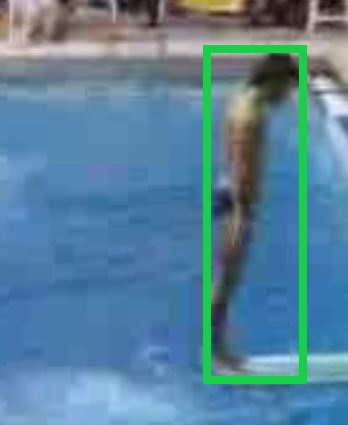
\includegraphics[width=\linewidth]{images/tracking/challenge_lowResolution}
		\caption{Images with low resolution.}
		\label{fig:challenge_lowResolution}
	\end{subfigure}
	\begin{subfigure}[!h]{0.54\textwidth}
		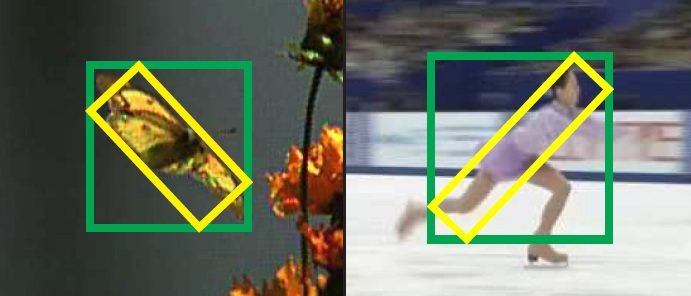
\includegraphics[width=\linewidth]{images/tracking/challenge_deformation}
		\captionsetup{margin=0.5cm}
		\caption{Two subject that can vary their appearance very quickly.}
		\label{fig:challenge_deformation}
	\end{subfigure}
	\begin{subfigure}[!h]{0.24\textwidth}
		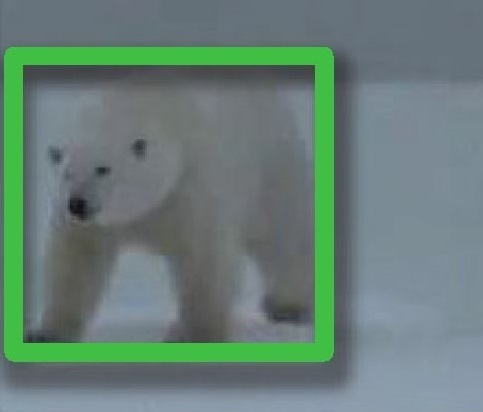
\includegraphics[width=\linewidth]{images/tracking/challenge_differentSubject}
		\caption{Tracking deals with objects, humans, and even animals.}
		\label{fig:challenge_differentSubject}
	\end{subfigure}
	%
	\begin{subfigure}[!h]{0.19\textwidth}
		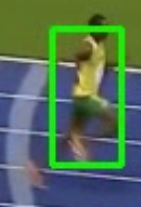
\includegraphics[width=\linewidth]{images/tracking/challenge_blurred}
		\caption{The limbs disappears.}
		\label{fig:challenge_blurred}
	\end{subfigure}
	\begin{subfigure}[!h]{0.49\textwidth}
		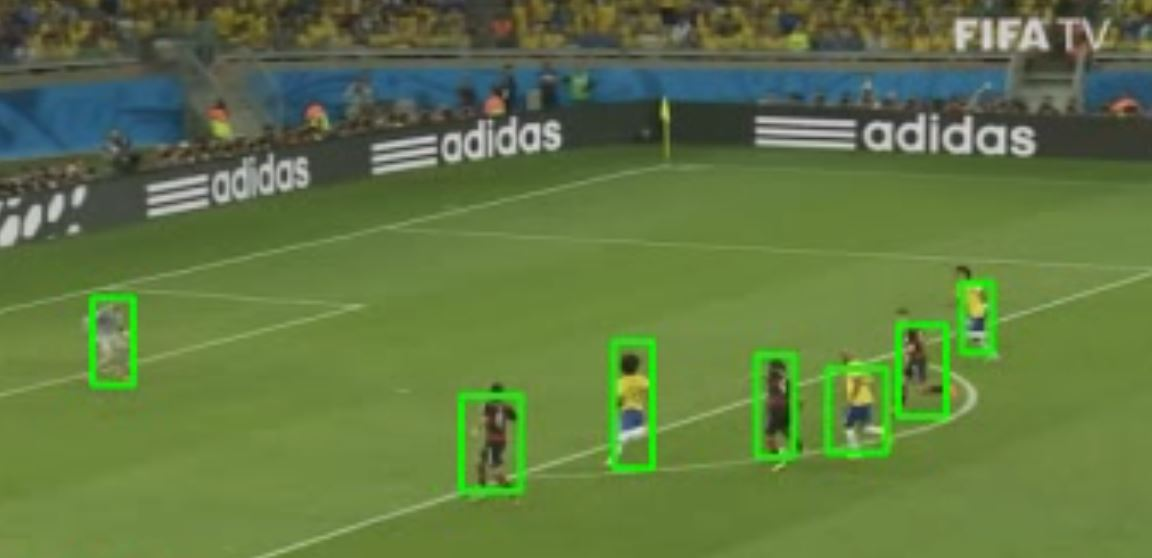
\includegraphics[width=\linewidth]{images/tracking/challenge_multiple}
		\captionsetup{margin=0.5cm}
		\caption{A soccer match action where all the players are tracked.}
		\label{fig:challenge_multiple}
	\end{subfigure}
	\begin{subfigure}[!h]{0.29\textwidth}
		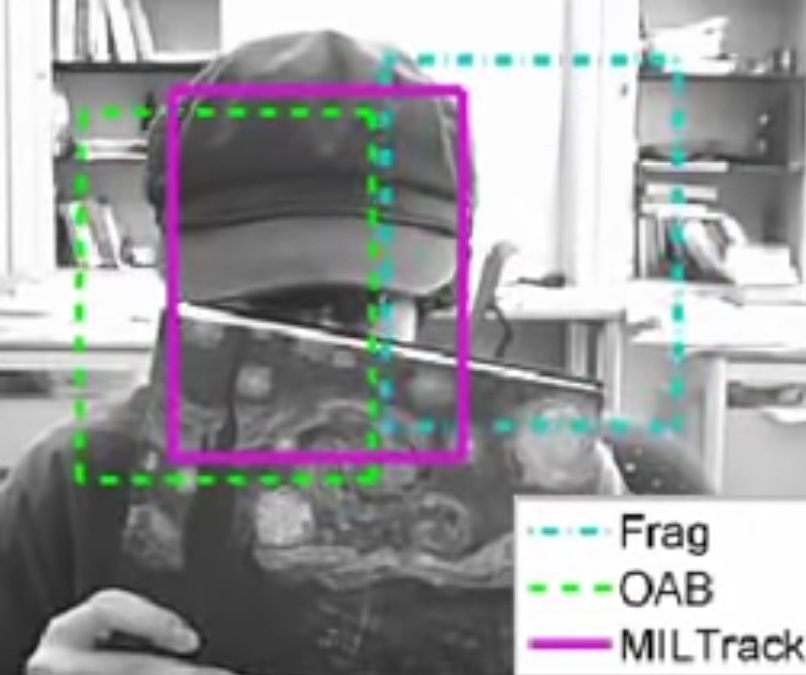
\includegraphics[width=\linewidth]{images/tracking/challenge_partialOcclusion}
		\caption{A face partially hidden by a hat and a book.}
		\label{fig:challenge_partialOcclusion}
	\end{subfigure}
	%
	\begin{subfigure}[!h]{0.49\textwidth}
		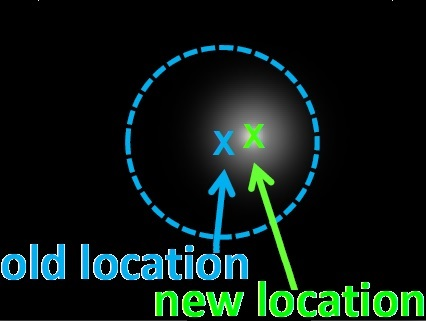
\includegraphics[width=\linewidth]{images/tracking/challenge_proximity}
		\caption{The new location is close to the older one.}
		\label{fig:challenge_proximity}
	\end{subfigure}
	\begin{subfigure}[!h]{0.49\textwidth}
		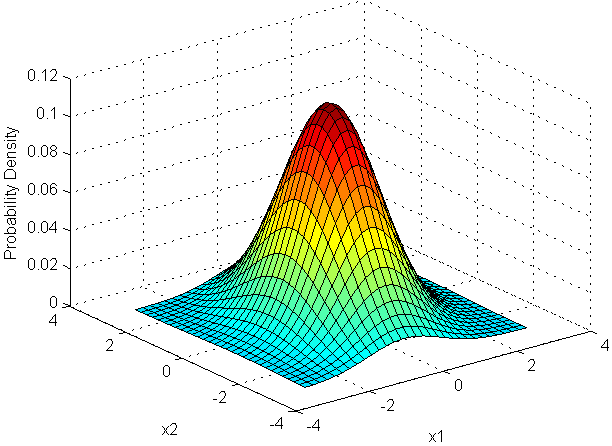
\includegraphics[width=\linewidth]{images/tracking/challenge_multivariate}
		\captionsetup{margin=0.5cm}
		\caption{The probability of where the new location is respect a multivariate normal distribution.}
		\label{fig:challenge_multivariate}
	\end{subfigure}
	%
	\begin{subfigure}[!h]{1\textwidth}
		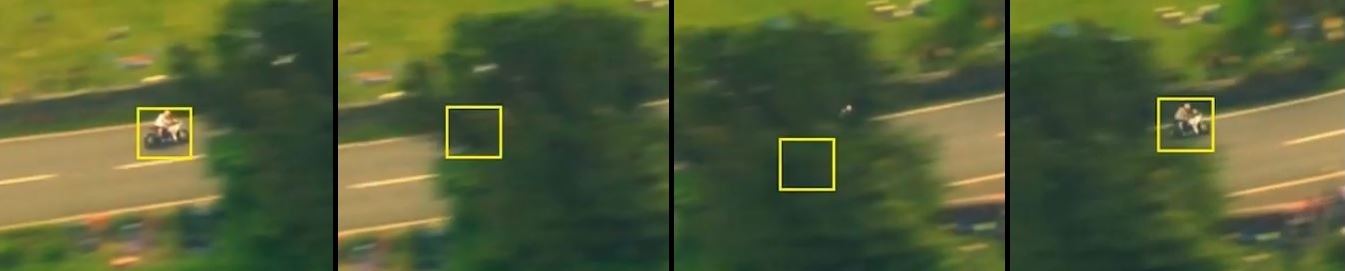
\includegraphics[width=\linewidth]{images/tracking/challenge_totalOcclusion}
		\caption{A motorcycle running on a street, is totally hidden by a tree for multiple frames.}
		\label{fig:challenge_totalOcclusion}
	\end{subfigure}
	\caption{Some visual examples of the tracking challenge conditions.}
	\label{fig:trackingChallenges}
\end{figure}


\subsection{The traditional tracking problem compared to the thesis project} \label{sec:trackingBaseliveVsThesis}
Some of the aspects explained in the previous section are extremely frequent in a lot of videos and databases, hence they are considered as a normal scenario. Others instead are often not even considered in the samples and the majority of the algorithms do not officially solve them.
\begin{itemize}
	\item The conditions that are often respected in object tracking are:
	\begin{itemize}
		\item The low-resolution images to allow the elaboration even without powerful computation devices, such as a smartphone. 
		\item A moving camera because a great majority of videos are in movement and shaking, except for the video surveillance field where the video camera is placed.
		\item The changes of 2D shape and the fast-moving objects should be respected, the robustness on these two points make the algorithms more or less reliable. 
		\item A short-time total occlusion might sometimes be managed, but it is rarely guaranteed.
	\end{itemize}

	\item The requirements for this thesis, except the traditional ones, are:
	\begin{itemize}
		\item Long-time occlusion. In our scenario where the robot physically follows a person, the leader can disappear behind a corner and will be hidden as long as the robot reaches it.
		\item Real-time processing. We have decided that to understand the movements in the real environment is sufficient a processing speed of 5 FPS.
		\item Long-term video. The algorithm is designed to last for a very long period, no explicit bounds exist since the drift problem has been solved.
		\item Subject limited to people. We are not interested in following animals or vehicles, even if extending the algorithm to them only require to change the object detectors setup and the internal database of images to train the recognition procedure.
	\end{itemize}
	
\end{itemize}



\section{Principal known algorithms}
In this section a set of algorithms that perform well to solve the tracking task is presented.\\
Differently, from object detection, the number of existing methods for tracking is much wider. This happens due to the high variability of the problem. The methods shown below represent a trade-off in terms of speed and reliability.


\subsection{MIL (Multiple Instance Learning) tracker}
The MIL tracker\cite{mil}\cite{mil-robust} is an extension of the older \textbf{BOOSTING Tracker}\cite{boosting}, both methods are based on an \textbf{online classifier}. "\textit{Online}" means that the classifier is trained "\textit{on the fly}" during the execution of the algorithms and not in advance. This type of training does not allow to use thousands of images but very few. An application of this method is presented in~\Cref{fig:sample_MIL}.\\
The idea of the online classifier is to trust the initialization of the tracker and to use the initial bounding box as the first training sample. The negative samples are then generated taking rectangles that do not overlap the positive example. The classifier learns during the execution to recognise the tracked subject as positive and the rest as negative.\\
The frames after the first one are elaborated similarly. The positive subject is searched around the last known position and the classifier assigns a probability to each proposal. The box with the highest score is chosen as positive and it is used to continue the training of the classifier.\\
The novelty of MIL compared to BOOSTING is shown in~\Cref{fig:howItWorks_MIL}).\\
Instead of using only the positive sample to fit the online classifier, MIL creates a bunch of bounding boxes proposals around the positive sample, called \textbf{bags}. All these boxes should contain the subject and one could even be perfectly centred on it. The training is done with the "Multiple Instance Learning" that takes the bag of positive proposals and selects the best one (the more centred one) to improve the classifier. In the end, the instance is trained with only one box that was chosen starting from a set of good alternatives and not with all of them. The negative samples are then generated as for the first frame.

\begin{figure}[!h]
	\centering
	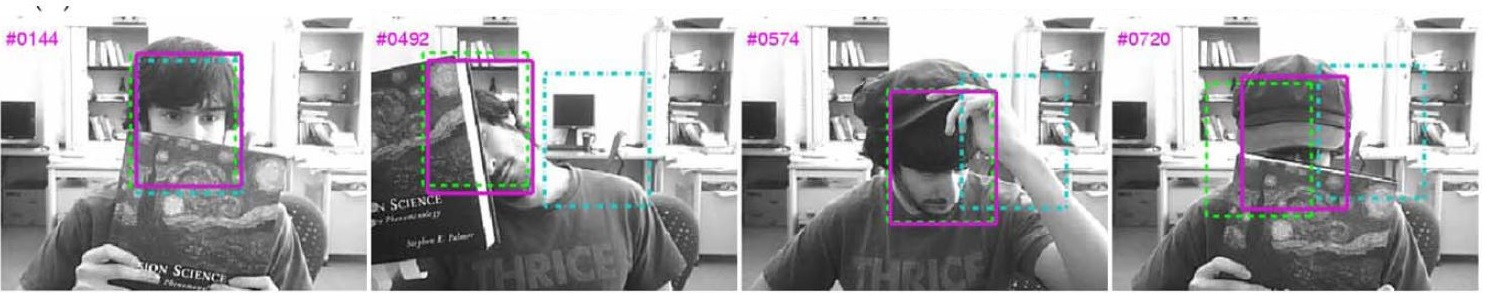
\includegraphics[width=1\linewidth]{images/tracking/sample_MIL}
	\captionsetup{margin=0.5cm}
	\caption[Examples of partial occlusion tracking.]{A sample of the MIL classifier tracking the face of the author while is partially occluded by a book. MIL tracker is in purple, while \textbf{\textcolor{cyan}{cyan}} and \textbf{\textcolor{green}{green}} are respectively FragTrack\cite{fragTrack} and Online Ada-Boost\cite{onlineAdaBoostTracker}.}
	\label{fig:sample_MIL}
\end{figure}
\begin{figure}[!h]
	\centering
	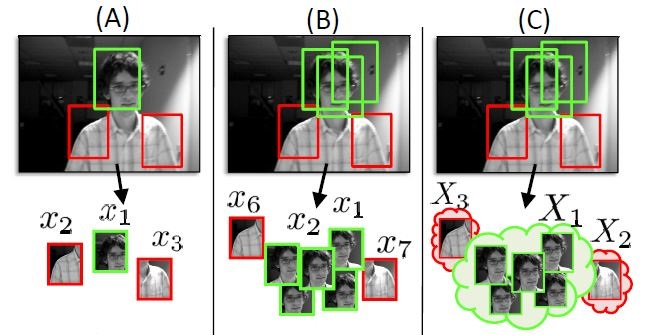
\includegraphics[width=0.8\linewidth]{images/tracking/howItWorks_MIL}
	\captionsetup{margin=0.5cm}
	\caption[The bag of bounding boxes introduced as MIL novelty.]{A comparison of how positive and negative samples are selected, to train the online classifier. In A the selection of BOOSTING tracker, the positive sample is used. In B a set of proposals generated around the positive are all used to train. In C the selection of MIL tracker, bags of samples are used and only one proposal is extracted and accepted from each one.}
	\label{fig:howItWorks_MIL}
\end{figure}


\subsection{KCF (Kernelized Correlation Filters) tracker} \label{sec:kcf}
The KCF tracker\cite{kcf}\cite{kcf-withColor} is an additional extension of MIL tracker.\\
The key idea is that the sampled images are similar due to the subject that is repeated or thanks to the background that does not change extremely fast compared to the FPS of the video. This repetition of similar patterns can be used to optimize the operations and speed up the computation. The technical improvement comes from the application of the \textbf{FFT (Fast Fourier Transformations)}, which allows to apply the elaboration of images in an efficient manner.\\
The novelty introduced with KCF allows this algorithm to outperform both BOOSTING and MIL, in terms of accuracy and speed. The weakness of this chain of three methods is the full occlusion. None of them is able to deal with total occlusion that always causes the tracking failure.


\subsection{Median Flow tracker} \label{sec:medianflow}
The Median Flow tracker\cite{medianFlow} is a reliable method that locates the subject according to its trajectory. The key idea is that the algorithm recognises points in two subsequent frames. These points should be the same physical element in the real space.\\
The overall procedure is shown in~\Cref{fig:howItWorks_medianFlow}. The first step (\Cref{fig:howItWorks_medianFlow_points}) consists of the creation of a grid of points on the initial bounding box, and then the localization of these points in all the future frames. This connection through the frames helps to know the exact motion model of the tracked algorithm. The \textbf{Motion Model} ($MM$) is the combination of actual position ($x, y$) and velocity. It is defined with the angle or direction of motion ($\theta$) and the module of the speed ($s$). Essentially knowing how the subject is moving helps to predict where it will be in the near future.
$$MM = ((x, y), (\theta, s))$$
The interaction of the frames works as follows. Every time that a new frame is added, the knowledge of the motion model suggests where the subject can be located. Then, the key points are searched in this new image. Once they are found it is fundamental to check the consistency of the trajectories (\Cref{fig:howItWorks_medianFlow_trajectory}). Each new point is associated with the most similar already known physical point and vice versa. If this double matching is correct and the two points refer to the same physical element the trajectory is confirmed (point 1 in the figure), otherwise there is a misalignment in the trajectories (point 2 in the figure). In~\Cref{fig:howItWorks_medianFlow_trajectory} point 2 is firstly (forward pass) associated with the front wheel, in the frame after is linked to the back wheel since the other one is hidden from the street signal. The backward pass links the back wheel again on itself. This misalignment of the connection is recognised as an error and so the point cannot be trusted. If no point can be trusted the tracking fails.\\
\\
Thanks to this double-checking procedure, the Median Flow tracker is a method that is able to well recognise when the tracking has failed to follow the subject. Unfortunately, the requirement to match key points over and over in the frames reduces the capability of the algorithm to manage scenarios where the subject appearance change too much.\\
For this reason, this algorithm is not good for tracking high deformable subjects such as animals and humans.

\begin{figure}[!h]
	\centering
	\begin{subfigure}{0.49\textwidth}
		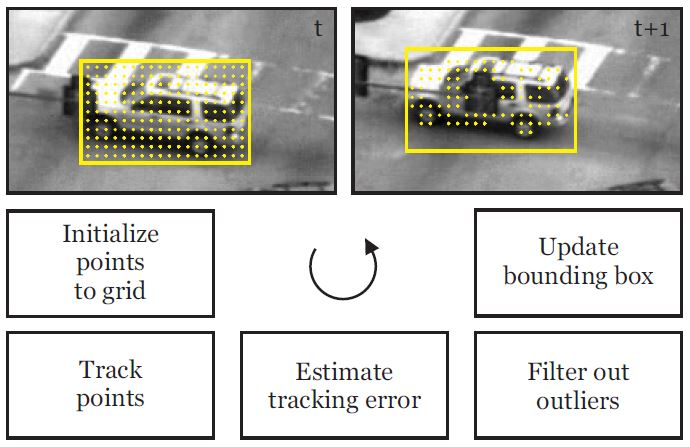
\includegraphics[width=\linewidth]{images/tracking/howItWorks_medianFlow_points}
		\captionsetup{margin=0.5cm}
		\caption{The first bounding box is divided into a grid of points, and a portion of them are recognised in the next frame. Below, the main steps of the algorithm.}
		\label{fig:howItWorks_medianFlow_points}
	\end{subfigure}
	\begin{subfigure}{0.49\textwidth}
		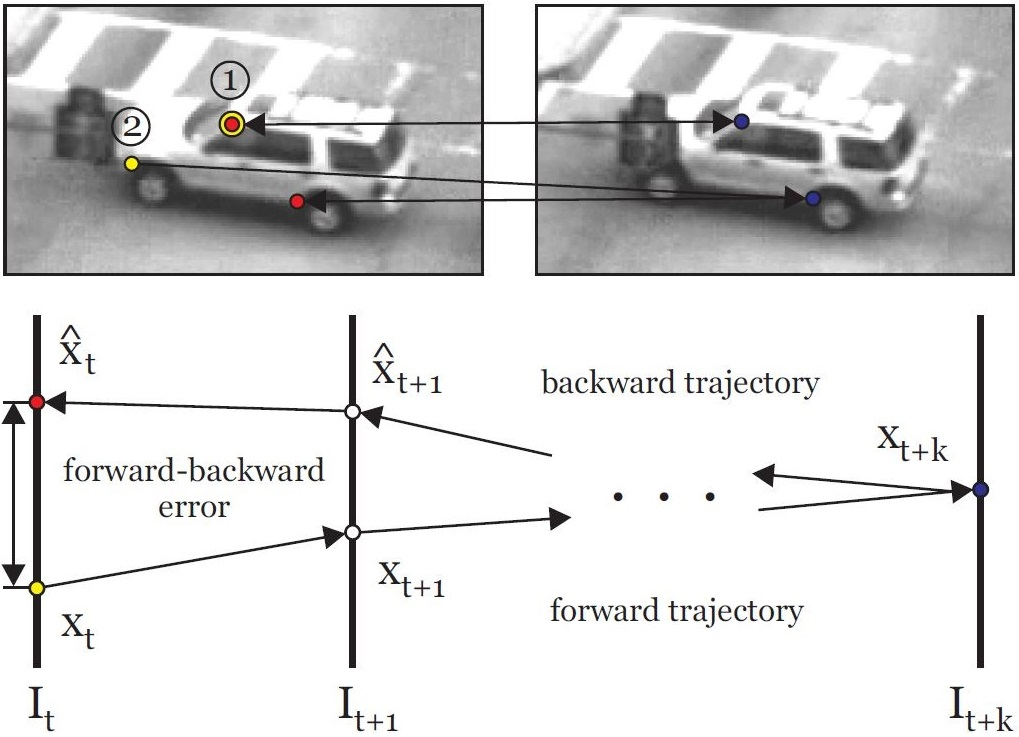
\includegraphics[width=\linewidth]{images/tracking/howItWorks_medianFlow_trajectory}
		\captionsetup{margin=0.5cm}
		\caption{The points found in two consecutive steps are compared to check if the forward and backward trajectories are the same and then it can be trusted.\\ Point 1 is accepted while point 2 is rejected.}
		\label{fig:howItWorks_medianFlow_trajectory}
	\end{subfigure}
	\captionsetup{margin=0.5cm}
	\caption[The key principle of the Median Flow tracker algorithm.]{The overall procedure of the Median Flow tracker computing forward and backward trajectories to precisely locate the target.}
	\label{fig:howItWorks_medianFlow}
\end{figure}


\subsection{CSRT (Channel and Spatial Reliability Tracker)}
The full name of the method is Discriminative Correlation Filter with Channel and Spatial Reliability (DCF-CSR)\cite{csrt}. Such as KCF (\Cref{sec:kcf}) and others, even this method is based on correlation filters.\\
\\
A \textbf{cross correlation filter} is a technique that aims at localizing into an image the exact position of another one. A representation of the cross-correlation usage done by CSRT is shown in~\Cref{fig:howItWorks_CSRT}. In details, the portion of the last frame, delimited by the last known bounding box, is elaborated with multiples correlation filters, each one producing a different output. These elaborations simulate possible changes in the appearance of the subject. Designing good filters is fundamental to well match the variability of the tracked subject and the generated features. The filter outputs are modified images of the last bounding box cropped area.\\
The output of each filter (an image) is moved along the full picture pixel by pixel (learning stage:~\Cref{fig:howItWorks_CSRT} left) to check which portion of the entire camera view is more probable the subject that we are looking for. The result of this scan is a confidence map that should present a peak in correspondence of the new position of the tracked subject.\\
All the filters can then be summed up together (localization stage:~\Cref{fig:howItWorks_CSRT} right) to highlight the proposal of each one and comes out with the final response. This response shows exactly where the subject is placed in the new frame.\\
\\
The characterization of CSRT is focused on the type of correlation filters used, with the idea of using a lot of them and combine the results at the end to produce a more reliable localization. The very high accuracy that this algorithm offers is compensated by the low FPS rate that it achieves.

\begin{figure}[!h]
	\centering
	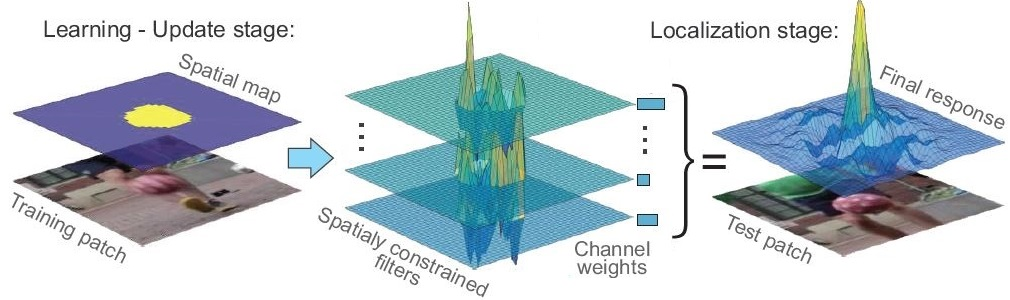
\includegraphics[width=1\linewidth]{images/tracking/howItWorks_CSRT}
	\captionsetup{margin=0.5cm}
	\caption[The general intuition of the CSRT algorithm.]{The overall procedure of the CSRT algorithm. The \underline{learning stage} is composed of multiple correlation filters that are applied to the input frame. Each filter produces a confidence map that highlights where the subject should be. The \underline{localization stage} combines all these confidence maps to produce the final response that precisely locates the subject.}
	\label{fig:howItWorks_CSRT}
\end{figure}
%\begin{figure}[!h]
%	\centering
%	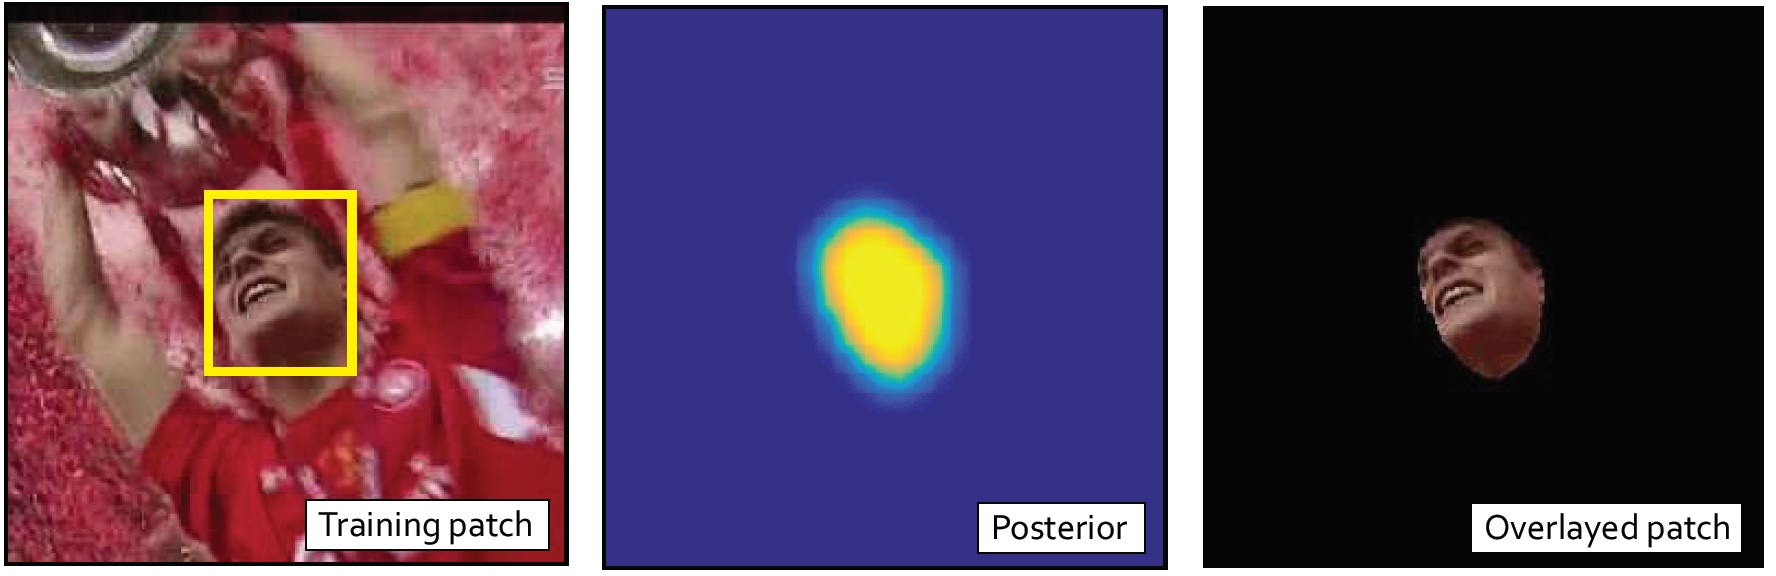
\includegraphics[width=0.8\linewidth]{images/tracking/sample_CSRT}
%	\captionsetup{margin=0.5cm}
%	\caption[An example of application of CSRT on a frame.]{A visualization of the confidence map applied to track the face of the man in the image. On the left the original image, centre the confidence map in 2D. On the right the cropped image according to localization.}
%	\label{fig:sample_CSRT}
%\end{figure}


\subsection{MOSSE (Minimum Output Sum of Squared Error) tracker}
The MOSSE algotihm\cite{mosse} such as KCF (\Cref{sec:kcf}) is a method whose strength lies into mathematical smart choices instead of a complex high-level logic like MedianFlow (\Cref{sec:medianflow}).\\
The novelty is introduced with a new correlation filter, called MOSSE. It can be applied to the input frames and precisely locate the variations fundamental to understand the movement of the subject.\\
Despite the original article states robustness against variations in lighting, scale and non-rigid deformations, this algorithm is not so reliable as it appears. On the other hand, the strength of this method is the extremely fast computations (FPS rate) that outperform all the other trackers presented in this section.

\subsection{GOTURN (Generic Object Tracking Using Regression Networks)} \label{sec:goturn}
GOTURN\cite{goturn} is a tracker based on neural networks. Differently from MIL and KCF (\Cref{sec:kcf}), this method is not based on an online NN, such as the online classifier, but it is based on an offline CNN.\\
An \textbf{offline NN} is a traditional NN that is trained on thousands of data: couples of images, in this case, producing the trained model. The process is done in advance, before the effective use, and not "on the fly" while running the tracker. The generated model is used at run time to know how to respond to an input value. The big advantage of offline methods is that the training procedure is the slowest section, for this reason an online classifier could not perform at very high FPS rates.\\
\\
The general workflow of the tracker is shown in~\Cref{fig:howItWorks_GOTURN}. The tracker takes as input a frame at a time and always compares it to the previous frame. This choice simplifies and standardizes the input to empower the potentiality of the CNN. However but makes the algorithm to have no chance against total occlusions even for one single frame. The CNN takes as input two squared images cropped from the frames. The crop on the previous frame is a bounding box centred around the last known position with some margins that will contain even the location in the frame afterwards. The current frame is cropped based on the same bounding box, but in this case, the subject is not centred in the square.\\
Then, both squared images are processed with two independent stacks of convolutional layers, followed by three fully-connected layers. The final output is composed of four values representing the top-left and bottom-right corners of the bounding box. It is centred on the subject in the squared image of the current frame. Some examples of the application of the CNN are shown in~\Cref{fig:sample_GOTURN}.

\begin{figure}[!h]
	\centering
	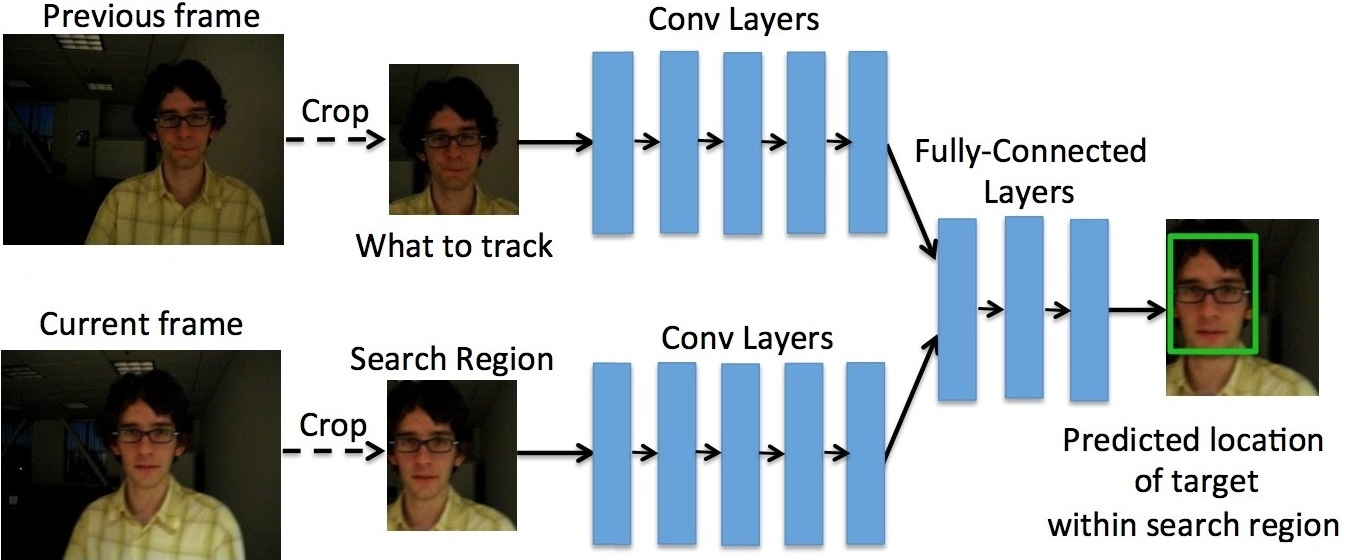
\includegraphics[width=0.9\linewidth]{images/tracking/howItWorks_GOTURN}
	\captionsetup{margin=0.5cm}
	\caption[The overall procedure of the GOTURN algorithm.]{The overall procedure of the GOTURN algorithm. On the left, the frames coming from the camera are cropped with the same square, that is centred on the subject in the previous frame (above). The images are elaborated with CNN to produce the output bounding box, that highlights where the subject is in the current frame.}
	\label{fig:howItWorks_GOTURN}
\end{figure}
\begin{figure}
	\centering
	\begin{minipage}{.62\textwidth}
		\centering
		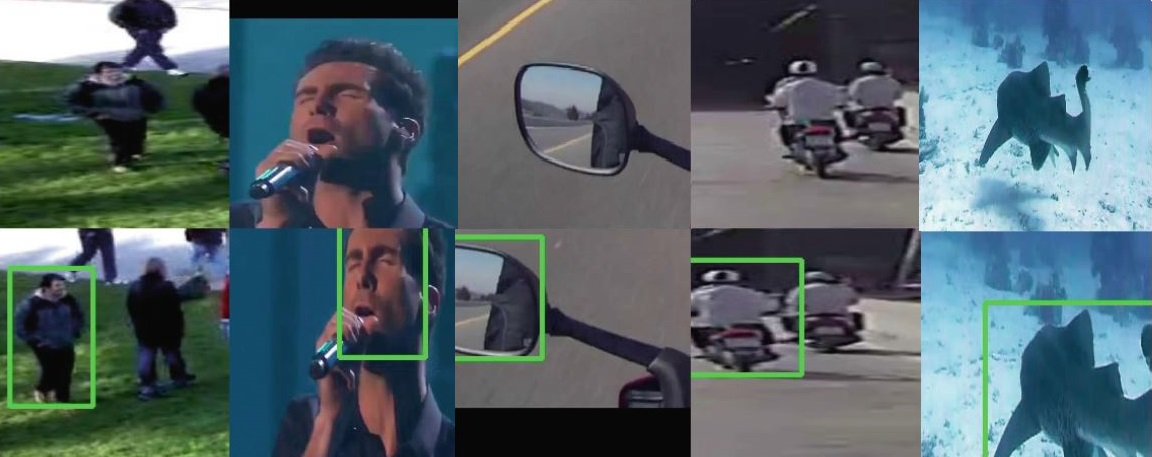
\includegraphics[width=1\linewidth]{images/tracking/sample_GOTURN}
		\captionsetup{margin=0.5cm}
		\captionof{figure}[Examples of application of the GOTURN algorithm.]{Samples of application of the CNN of GOTURN. The two squared images coming from previous (above) and current (below) frame are fed into the network. The answer is the \textbf{\textcolor{green}{green}} bounding box that locates the tracked subject on the new frame.}
		\label{fig:sample_GOTURN}
	\end{minipage}
	\hspace{0.03\linewidth}
	\begin{minipage}{.32\textwidth}
		\centering
		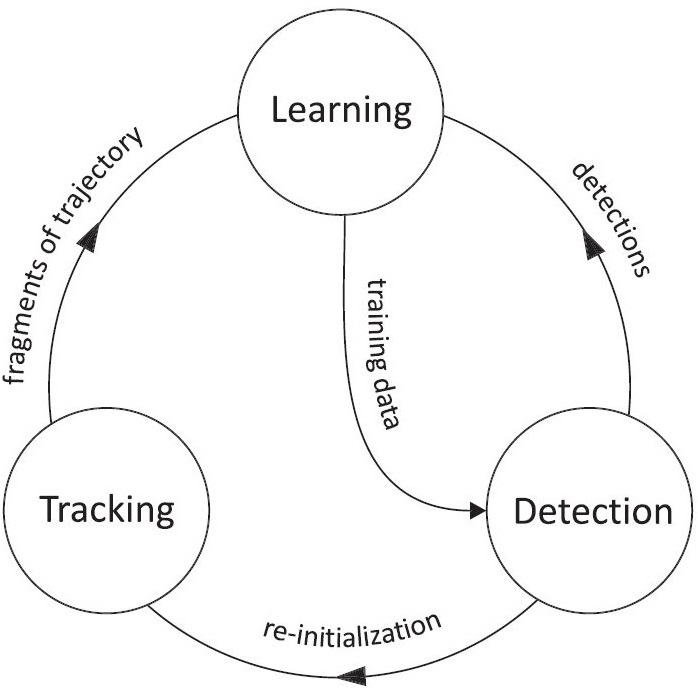
\includegraphics[width=1\linewidth]{images/tracking/howItWorks_TLD}
		\captionof{figure}{The interconnection of the three foundation methods of TLD algorithm.}
		\label{fig:howItWorks_TLD}
	\end{minipage}
\end{figure}


\subsection{TLD (Tracking-Learning-Detection)} \label{sec:tld}
Differently from all the other methods, TLD\cite{tld} aims to be a complete tracker able to deal with extremely complex scenarios. If the previously presented trackers have no chance to manage a long-time total occlusion and a long-term tracking, this method is able to overcome both of the problems. A sample showing potentiality is in the~\Cref{fig:sample_TLD}.\\
The foundation principle is that TLD is not a single algorithm but it is a combination of three. The interaction of these three parts is shown in~\Cref{fig:howItWorks_TLD}. The key idea to overcome the re-identification problem that occurs after a total occlusion, or the drift problem that happens along a large video, is to often re-initialize the tracker. In fact, the \underline{tracking} (\textbf{T}) of TLD aims at managing short-term video clips. When a small problem occurs the \underline{detection} (\textbf{D}) tries to locate the subject back again. While these two situations take turns, the \underline{learning} procedure (\textbf{L}) extracts the key elements that recognise uniquely the subject and understand how to precisely locate it inside the frame.\\
\\
The trade-off to use this extremely flexible structure is paid with a not high FPS rate. However, the biggest problem of this method is the huge quantity of false-positive predictions. The learning procedure starts with a few samples, meaning that errors in the beginning phase can occur easily. The failure in the first phase causes wrong learning that will produce more and more errors later on.\\
Despite the good potentialities, this algorithm is not reliable for the traditional tracking task.
\begin{figure}[!h]
	\centering
	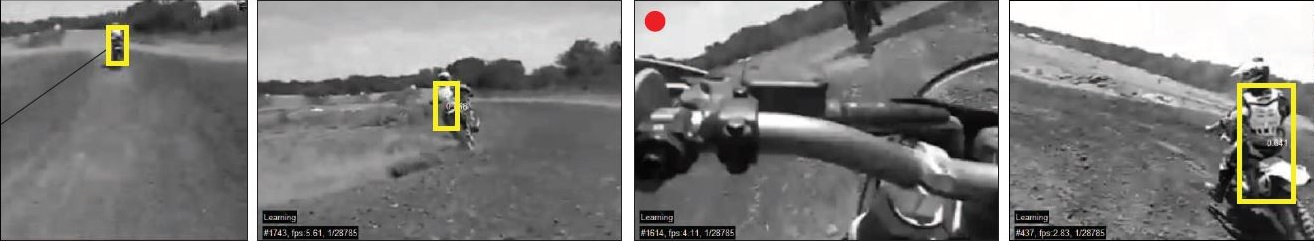
\includegraphics[width=.9\linewidth]{images/tracking/sample_TLD}
	\captionsetup{margin=0.5cm}
	\caption[TLD algorithm applied on a total occlusion video clip.]{A sample that shows the potentialities of the TLD algorithm, dealing with a total occlusion while tracking a motorbike with a dramatic change of size. The \textbf{\textcolor{red}{red}} dot means that the subject cannot be found.}
	\label{fig:sample_TLD}
\end{figure}



\section{Which tracker could be chosen}
In the previous section we have presented seven different tracking algorithms, each one with his own strengths and weaknesses. These methods are the ones that were explored during this thesis work, but many others exist.\\
The tracking task that we aim at solving is a long real-time sequence with long-lasting total occlusions, as explained in~\Cref{sec:trackingBaseliveVsThesis}. This task is solved with a combination of detection, tracking and recognition, so the internal tracking challenge is much simpler.\\
The requirement is to solve the baseline tracking task (\Cref{sec:tracking-definition}), and to deal with changes of shape and partial occlusions. Considered the explained methods and known their speed performances (shown in~\Cref{tab:trackersFPS}), here it is what we have chosen. Note that the underlined methods are the best trade-off choices. 
\begin{itemize}
	\item \textbf{MIL tracker} is not a good choice because it runs at few FPS and a newer version that outperforms both its speed and accuracy exists.
	\item \underline{\textbf{KCF tracker}} is the new version of MIL. It is one of the fastest methods and it is also reliable. It suffers the rapid change of appearance and, less important for our scenario, it does not manage total occlusions.
	\item \textbf{Median Flow tracker} works well only on not deformable or rigid subjects. Since we are dealing with humans it is a bad choice.
	\item \underline{\textbf{CSRT}} is the most reliable method, it could even manage short total occlusions. Despite the low FPS rate is a great choice, in fact, our goal is a tracker running at around 5 FPS that is way less than the speed of CSRT.
	\item \underline{\textbf{MOSSE}} is focused on pure speed. It is not the most reliable method but it can be a good choice to try to reach the highest FPS rate for the general challenge.
	\item \underline{\textbf{GOTURN}} is a reliable method, running at a good FPS rate. At the moment it is not integrated in this project but it can be a great choice for future improvements.
	\item \textbf{TLD} is a too complex method. It is able to solve long total occlusions but easily fails on simpler scenarios, by proposing a lot of false positives. It is not reliable at all for our purpose.
\end{itemize}
Note that the principle proposed in this thesis is similar to the one of which TLD is based. The integration of tracking and detection linked together with a third procedure: learning in case of TLD and person recognition for this project. Both algorithms aim at solving the total occlusion problem and the drift problem with a reinitialization of the tracker performed with an object detector. The key difference is the existence in this thesis of the \textit{slow start} phase presented in~\Cref{sec:slowStartPhase}.

\begin{table}[]
	\centering
	\begin{tabular}{|c|c|c|c|c|c|c|c|}
		\hline
		Algorithm & MIL & KCF & MedianFlow & CSRT & MOSSE & GOTURN & TLD \\ \hline
		FPS  & 9   & 38  & 40         & 15   & 56    & 20     & 10  \\ \hline
	\end{tabular}
	\captionsetup{margin=0.5cm}
	\caption[The FPS rates of the tracking algorithms.]{An overview of the FPS rate of the trackers described. The performances were measured on an Intel Core i5 CPU and on an Nvidia Jetson TX2 GPU. The speeds measured are almost the same.}
	\label{tab:trackersFPS}
\end{table}